\documentclass[twocolumn,showpacs,floatfix,nofootinbib,longbibliography]{revtex4-1}
\usepackage{graphicx}
\usepackage{bm} % bold math
\usepackage{amssymb} % use this package to enable \nrightarrow command
\usepackage{amsmath} % use this package to enable \xrightarrow command
\usepackage{braket} % use for Dirac bra-kets : \rangle \labgle & \mid
\usepackage{natbib} % bibtex package
\usepackage{hyperref}


\begin{document}

\title{Skyrmion-induced localized state in a two-dimensional superconductor}

\author{Sho Nakosai$^{1,2}$}
\author{Sergey S. Pershoguba$^{1}$}
\author{Alexander V. Balatsky$^{1,3}$}
\affiliation{$^1$Nordita, Center for Quantum Materials, KTH Royal Institute of Technology, and Stockholm University, Roslagstullsbacken 23, S-106 91 Stockholm, Sweden}
\affiliation{$^2$Department of Applied Physics, University of Tokyo, Tokyo 113-8656, Japan}
\affiliation{$^3$Institute for Materials Science, Los Alamos National Laboratory, Los Alamos, NM 87545, USA}

\date{\today}


\begin{abstract}
We consider a superconductor proximity coupled to a 2D ferromagnetic film with a topological configuration of the ferromagnetic vector, i.e. the skyrmion. Using the T-matrix calculations as well as well numerical modeling we calculate the spin-polarized local density of states (SP-LDOS) in the vicinity of the skyrmion. We identify a skyrmion-induced Yu-Shiba-Rusinov (s-YSR) bound state, calculate its energy and a spectral width. We predict that sYSR resonance has a spatial power-law decay. This implies that superconductivity could facilitate a long-range interaction between distinct skyrmions on the surface of the ferromagnetic film.
\end{abstract}

\pacs{ }   

%%%%%%%%%%%%%%%%%%%%%%%%%%%%%%%%%%%%%%%%%%%%%%%%%%%%%%%%%%%%%%%%%%%%%%%%%%

\maketitle
%%%%%%%%%%%%%%%%%%%%%%%%%%%%%%%%%%%%%%%%%%%%%%%%%%%%%%%%%%%%%%%%%%%%%%%%%%%
\paragraph*{Introduction.} \label{sec:intro}
%%%%%%%%%%%%%%%%%%%%%%%%%%%%%%%%%%%%%%%%%%%%%%%%%%%%%%%%%%%%%%%%%%%%%%%%%%%

General context of skyrmions asd tolopolical excitations: memory, manipulation, local creation via SP STM.
Extension of skyrmion discussion to the case of hybrid structures: SC and Skyrmion. What are the consequenc of brining topological exchange field into SC. Question we address is the possible local spectroscopic signatures of SC quasiparticles in SC due to skyrmion field. We know from the past discussion that there are impurity bound states in SC near magnetic impurities. We have now the framework to address formation of bound states. Talk about local single impurity limit (YSR) and show the cartoon of the local and extended skyrmion and spectra. There are two effects: local scattering and Zeeman field hence the DOS will be split etc.  Draw similarities and differences with single imp.
In parallel with skyrmion discovery the local imaging using magnetic probes like MFM and SP-STM allowed one to image the matter at atomic resolution while also resolving spin content of electron carriers in the substrate.  
Here we prove the existence of the new type of localized excitation on the skyrmion core we call  Sc-YSR state (alternative is skyrmion bound state (sbs)).  Show the main results upfront in the introduction. Both LDOS and SP-LDOS. 
Main section: 

It has been pointed out over the past few years that superconductivity can facilitate strong long-range interaction between the magnetic impurities. Maybe the same thin will happen for skyrmions. 

Skyrmions in Wiesendanger's group \cite{Heinze2011,Romming2013,Bergmann2014,Brede2014,Sonntag2014,vonBergmann2015,Romming2015}.
.


Introduce T matrix and results for analytic solution.  
Introduce the numerical approach and presenst the results oas a function of position and as a function of energy. Kind of same figs as in Sho’s talk. 
Discuss the results and what it means, how big the signal is etc. Unfortunately we do not see any topological state at zero energy and as such these result represent a new kind of magnetic texture induced states that exhibit intragap states.



%%%%%%%%%%%%%%%%%%%%%%%%%%%%%%%%%%%%%%%%%%%%%%%%%%%%%%%%%%%%%%%%%%%%%%%%%%%
\paragraph*{Skyrmions in ferromagnetic films.} \label{sec:skyrmion}
%%%%%%%%%%%%%%%%%%%%%%%%%%%%%%%%%%%%%%%%%%%%%%%%%%%%%%%%%%%%%%%%%%%%%%%%%%

%%%%%%%%%%%%%%%%%%%%%%%%%%%%%%%%%%%%%%%%%%%%%%%%%%%%%%%%%%%%%%%%%%%%%%%%%%%
\begin{figure} \centering
(a) 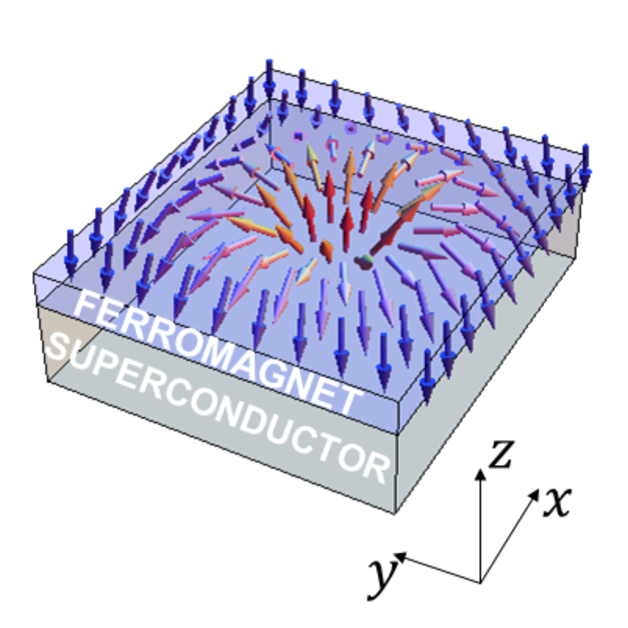
\includegraphics[width=0.4\linewidth]{SkyrmA}  
(b) 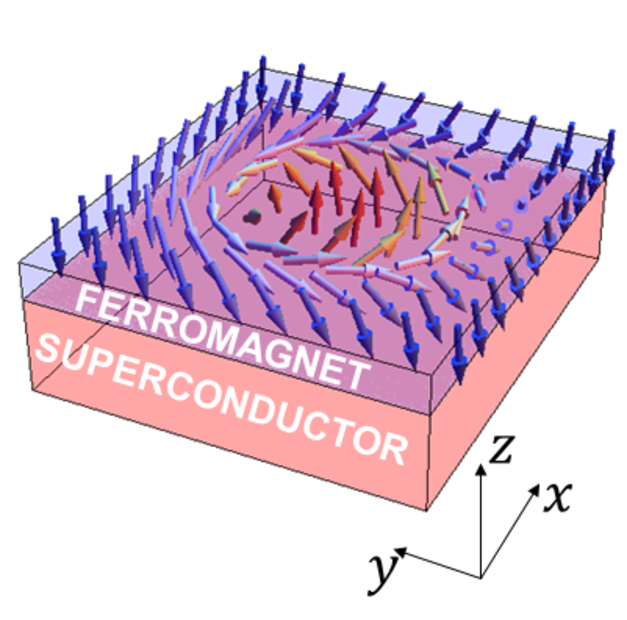
\includegraphics[width=0.4\linewidth]{SkyrmB} 
\caption{(Color online.) Ferrormagnetic film deposited on top of a superconductor. The ferromagnetic vector has skyrmion configuration. (a) Hedgehog skyrmion.  (b) Spiral skyrmion. } \label{fig:skyrmion}
\end{figure}
%%%%%%%%%%%%%%%%%%%%%%%%%%%%%%%%%%%%%%%%%%%%%%%%%%%%%%%%%%%%%%%%%%%%%%%%%%


%%%%%%%%%%%%%%%%%%%%%%%%%%%%%%%%%%%%%%%%%%%%%%%%%%%%%%%%%%%%%%%%%%%%%%%%%%%
\begin{figure*} \centering
	(a)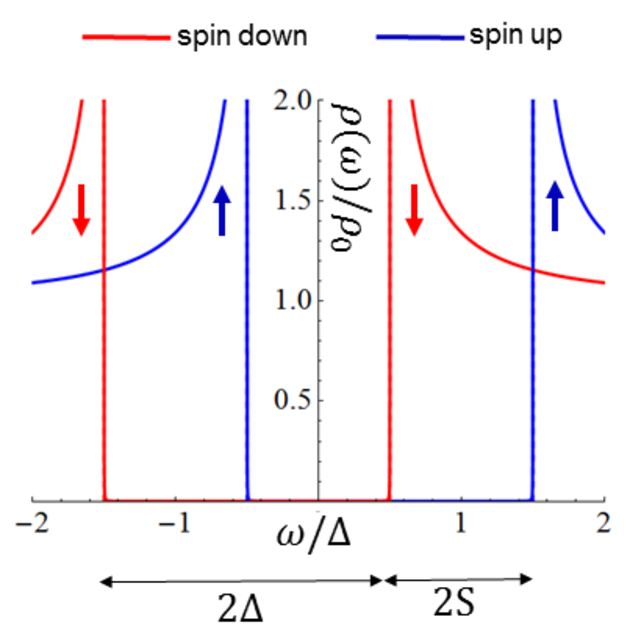
\includegraphics[width=0.25\linewidth]{LDOSa} \hspace{0.1cm}
	(b)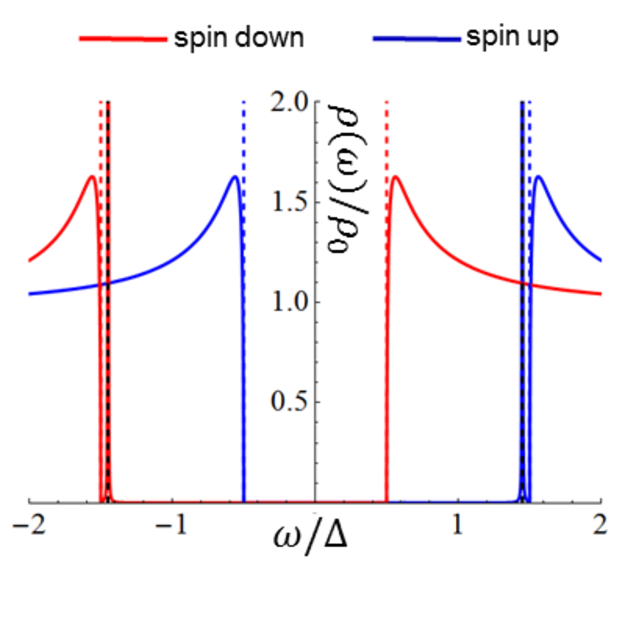
\includegraphics[width=0.25\linewidth]{LDOSb} \hspace{0.1cm}
	(c)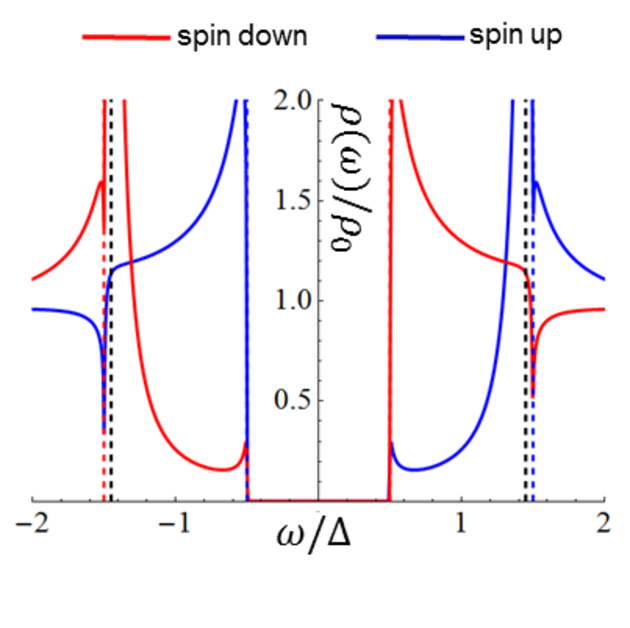
\includegraphics[width=0.25\linewidth]{LDOSc} 
\caption{(Color online) Spin-polarized local density of states (a) away from the skyrmion and (b,c) at the core of the skyrmion. Panel (b) corresponds to the usual T-matrix that takes into account only out-of-plane. Panel (c) corresponds to the T-matrix that takes into account in-plane spin. Comparing (b) and (c) notice that a thin YSR state in (b) becomes a thick resonance in (c). The parameters of plots are $2S = \Delta = 0.25 E_F$ and $R = 1/p_F = \xi/8$. Blue and red dashed lines indicate the positions of the shifted spin-up and spin-down bands, respectively. The black dashed line indicates the position of the YSR pole, given by Eq.~.} \label{fig:LDOS}
\end{figure*}
%%%%%%%%%%%%%%%%%%%%%%%%%%%%%%%%%%%%%%%%%%%%%%%%%%%%%%%%%%%%%%%%%%%%%%%%%%


Let the three-dimensional vector $S(\bm r) = (S_x,S_y,S_z)$ describe the configuration of the ferromagnetic vector in a two-dimensional ferromagnetic film $\bm r = (x,y)$. The configurations of the field $S(\bm r)$ shown in Fig. \ref{fig:skyrmion}(a) and (b) are referred to as skyrmions. The skyrmion configuration of the field is characterized by the topological charge 

\begin{align}
	Q = \frac{1}{4\pi} \int d^2r \, \hat {\bm S}\cdot (\nabla_x\hat {\bm S}\times\nabla_y\hat {\bm S}), \quad \hat {\bm S}= \frac{\bm S}{S}, 
	\label{topCharge}
\end{align}
which cannot be altered by the continuous transfomation of the field.  We also characterize the skyrmion fields by the zeroth and first moments
\begin{align}
	S^{(0)}_i = \int  d^2r \, \left[S_i(\bm r)-S_i(\infty)\right],\,\, i\in \{x,y,z\}, \label{S0} \\
	S^{(1)}_{ij} = \int  d^2r \, \left[S_i(\bm r)-S_i(\infty)\right] r_j,\,\, j\in \{x,y\}. \label{S1}
\end{align}
The zeroth moment $\bm S^{(0)} = S_{\rm e} \hat{\bm z}$ characterizes the effective out-of-plane magnetic moment of the skyrmion and is equal for the two skyrmions shown in Fig.~{\ref{fig:skyrmion}}(a) and (b). Whereas, the first-order moment $S^{(1)}_{ij}$ characterizes the in-plane pattern of the ferromagnetic vector $\bm S(\bm r)$. Note that for the cylindrically symmetric field $S(\bm r)$, the first order moment defined in Eq.~(\ref{S1}) can be expanded in the symmetric and antisymmetric parts 
\begin{equation}
	S^{(1)}_{ij}=S_{\rm m}\,\delta_{ij} + S_{\rm a}\,\epsilon_{ijz}
\end{equation}	
The skyrmions shown in Fig.~\ref{fig:skyrmion}(a) and (b) have monopole $S_{\rm m}$ and anapole $S_{\rm a}$ moments correspondingly, hence the name of the skyrmions. However the two types of the skyrmions have the same topological charge~(\ref{topCharge}) and thus can be continuosly deformed into each other. 

%%%%%%%%%%%%%%%%%%%%%%%%%%%%%%%%%%%%%%%%%%%%%%%%%%%%%%%%%%%%%%%%%%%%%%%%%%%
\begin{figure*} \centering
	(a)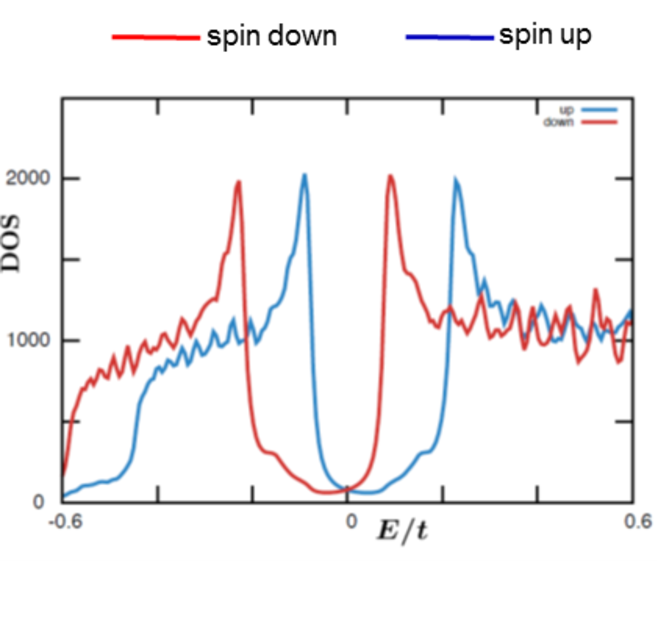
\includegraphics[width=0.25\linewidth]{numerical-LDOS-away} \hspace{0.1cm}
	(b)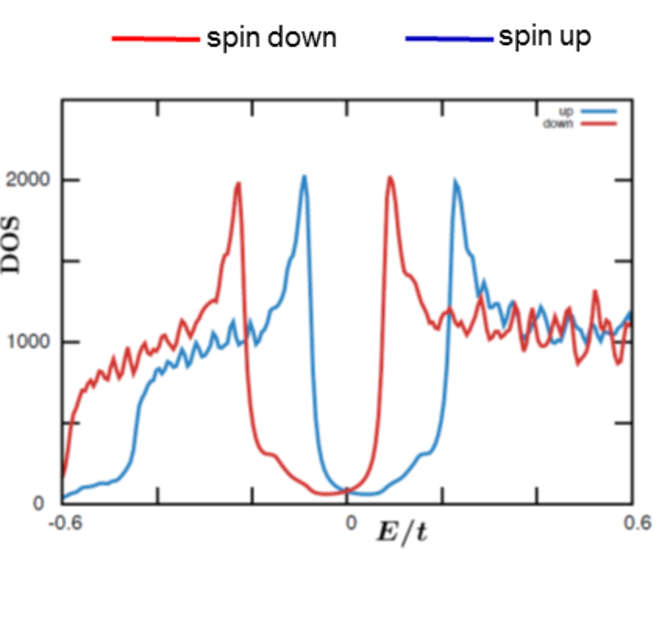
\includegraphics[width=0.25\linewidth]{numerical-LDOS-core} \hspace{0.1cm}
	(c)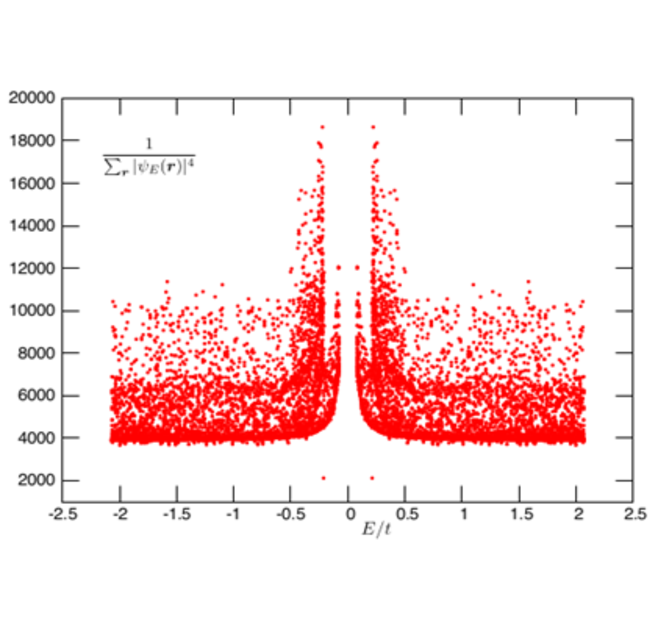
\includegraphics[width=0.25\linewidth]{numerical-IPR} 
\caption{(Color online) Numerical modeling of a skyrmion: (a) LDOS away from the skyrmion (PLEASE SUBSTITUTE WITH THE CORRECT FIGURE), (b) LDOS at the skyrmion core, (c) inverse participation ratio (IPR).} \label{fig:LDOSNumerics}
\end{figure*}
%%%%%%%%%%%%%%%%%%%%%%%%%%%%%%%%%%%%%%%%%%%%%%%%%%%%%%%%%%%%%%%%%%%%%%%%%%

%%%%%%%%%%%%%%%%%%%%%%%%%%%%%%%%%%%%%%%%%%%%%%%%%%%%%%%%%%%%%%%%%%%%%%%%%%%
\paragraph*{Model}  \label{sec:model}
%%%%%%%%%%%%%%%%%%%%%%%%%%%%%%%%%%%%%%%%%%%%%%%%%%%%%%%%%%%%%%%%%%%%%%%%%%
The model is given by the following 4-by-4 Bogolyubov-de Gennes (BdG) Hamiltonian 
\begin{align}
	 H &= \xi(\bm p)\tau_z+\Delta \tau_x - \bm S(\bm r)\cdot\bm\sigma, \label{ham} \\
  & \xi(\bm p) = \frac{p^2}{2m}-\mu,\quad \bm p = -i(\nabla_x,\nabla_y),
\end{align}
which describes the proximity coupling of the ferromagnetic vector $S(\bm r)$ to the itinerant electrons of a two-dimensional (2D) superconductor with the superconducting gap $\Delta$. The Pauli matrices $\bm \tau$ and $\bm \sigma$ act, respectively, in the particle-hole and spin subspaces of the four-component spinor $\Psi = (\psi_\uparrow,\psi_\downarrow,\psi^\dagger_\downarrow,-\psi^\dagger_\uparrow)^T$. For simplicity, we assume that the magnitude of the superconductor-ferromagnet coupling is constant and only the direction $\bm S(\bm r)$ varies, i.e. we set $\bm S(\bm r) = S\,\bm n(\bm r)$, where $\bm n$ is a unit vector. In order to proceed further let compare the typical lengthscales. The radius of skyrmions $R$ found in experiments~\cite{Heinze2011,Romming2013,Bergmann2014,Brede2014,Sonntag2014,vonBergmann2015,Romming2015} does not typically exceed $5$ nm, whereas the superconducting coherence length $\xi_{sc}$ varies largely from a micron to a few nanometers as in, e.g., curprates. For the analysis below, we assume the superconducting coherence length much larger $\xi_{sc}\gg R$, and briefly comment about the opposite limit in the Supplemental Material (Shall we discuss this? Local gauge transform and introduce effective spin-orbit, etc. ). In the chosen limit the superconductivity cannot ``resolve'' the fine details of the field $\bm S(\bm r)$ and only ``sees'' as a skyrmion as local magnetic defect. Therefore we shall apply a Yu-Shiba-Rusinov \cite{Yu,Shiba,Rusinov,Balatsky2006} treatment the skyrmion as a local impurity. 
%%%%%%%%%%%%%%%%%%%%%%%%%%%%%%%%%%%%%%%%%%%%%%%%%%%%%%%%%%%%%%%%%%%%%%%%%%%
\paragraph*{T-matrix analysis} \label{sec:analytics}
%%%%%%%%%%%%%%%%%%%%%%%%%%%%%%%%%%%%%%%%%%%%%%%%%%%%%%%%%%%%%%%%%%%%%%%%%%%
It is convenient to split the Hamiltonian~(\ref{ham}) $H = h(\bm p)+V(\bm r)$ into the spatially uniform part $h(\bm p)$ and a local perturbation $V(\bm r)$ describing the skyrmion
\begin{align}
	h(\bm p) & =  \xi(\bm p)\tau_z+\Delta \tau_x - \bm S(\infty)\cdot\bm\sigma,\quad \bm S(\infty) = -S\,\hat{\bm z}\\
	V(\bm r) & =  - \left[\bm S(\bm r)-\bm S(\infty)\right]\cdot\bm\sigma  \label{vr}
\end{align}
For the skyrmions shown in Figs.~\ref{fig:skyrmion}(a) and (b), the ferromagnetic vector is $S(\infty) = -S\,\hat{\bm z}$ far from skyrmion, and is parallel to $\bm S(0)= S\hat{\bm z}$ at the skyrmion core. The Hamiltonian $h(\bm p)$ describes a superconductor proximity coupled to a ferromagnet with constant magnetization, i.e. in the absence of the skyrmion. The ferromagnetic coupling merely shifts the bands corresponding the opposite spins as shown in Fig.~(\ref{fig:LDOS})(a). The spectrum maintains a gap as long as the Zeeman coupling is less than the superconducting gap, i.e. $S<\Delta$. Such spectrum should be possible to detect by the spin-polarized tunneling spectroscopy methods[cite relevant papers]. In the presence of the skyrmion, the term~(\ref{vr}) should be taken into account. As pointed out above, for small skyrmion size $\xi_{sc}\gg R$, the skyrmion field can be approximated as a local magnetic impurity with $S(\bm r)=\bm S_{\rm e}\,\sigma_z \delta^2(\bm r)$, where the effective magnetization is determined in Eq.~(\ref{S0}). Such a local perturbation can be  treated exactly by calculating the T-matrix
\begin{align}
	T(\omega) =   \frac{-S_{\rm e}\sigma_z}{1+S_{\rm e}\sigma_zg_{0}(\omega)} \label{tm} 
\end{align}
taken into account in T-matrix calculation, which gives the following SP-LDOS at the skyrmion core
\begin{align}
	\rho_s & (\omega) = \label{ldos} \\ 
	&-\frac{1}{\pi}\,{\rm Im}{\rm \,Tr} \left\{  \frac{1+\tau_z}{2}\,\frac{1+\sigma_s}{2} \left[g_0(\omega)+g_0(\omega) T(\omega) g_0(\omega)  \right]\right\},\nonumber 
 \end{align}
 where energy has infinitesimally small imaginary part in the right side of the equation, i.e. $\omega\rightarrow \omega+i\delta$, and $s=x,y,z$ denotes the spin quantization axis. We plot LDOS (\ref{ldos}) in Fig.~\ref{fig:skyrmion}(b).   


%%%%%%%%%%%%%%%%%%%%%%%%%%%%%%%%%%%%%%%%%%%%%%%%%%%%%%%%%%%%%%%%%%%%%%%%%%%
\paragraph*{Numerical analysis.} \label{sec:numerics} 
%%%%%%%%%%%%%%%%%%%%%%%%%%%%%%%%%%%%%%%%%%%%%%%%%%%%%%%%%%%%%%%%%%%%%%%%%%%

%%%%%%%%%%%%%%%%%%%%%%%%%%%%%%%%%%%%%%%%%%%%%%%%%%%%%%%%%%%%%%%%%%%%%%%%%%%
\begin{figure} \centering
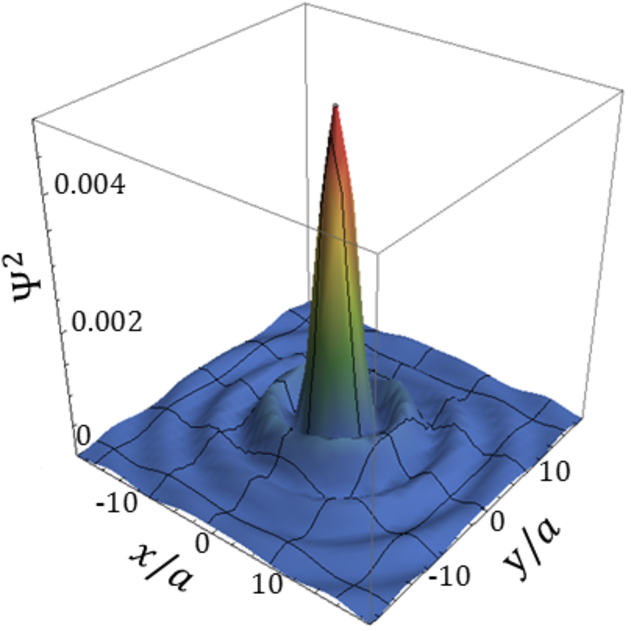
\includegraphics[width=0.7\linewidth]{WaveFunction}  
\caption{(Color online) Numerical wavefunction corresponding to the sYSR state. The wave function has pronounced oscillations with a period of approximately the superconducting coherence length.  } \label{fig:wavefunction}
\end{figure}
%%%%%%%%%%%%%%%%%%%%%%%%%%%%%%%%%%%%%%%%%%%%%%%%%%%%%%%%%%%%%%%%%%%%%%%%%%

%%%%%%%%%%%%%%%%%%%%%%%%%%%%%%%%%%%%%%%%%%%%%%%%%%%%%%%%%%%%%%%%%%%%%%%%%%%
\paragraph*{Discussion  } \label{sec:discussion} 
%%%%%%%%%%%%%%%%%%%%%%%%%%%%%%%%%%%%%%%%%%%%%%%%%%%%%%%%%%%%%%%%%%%%%%%%%%%



%%%%%%%%%%%%%%%%%%%%%%%%%%%%%%%%%%%%%%%%%%%%%%%%%%%%%%%%%%%%%%%%%%%%%%%%%%%
\paragraph*{Conclusion} \label{sec:conclusion}
%%%%%%%%%%%%%%%%%%%%%%%%%%%%%%%%%%%%%%%%%%%%%%%%%%%%%%%%%%%%%%%%%%%%%%%%%%%






\appendix 

%%%%%%%%%%%%%%%%%%%%%%%%%%%%%%%%%%%%%%%%%%%%%%%%%%%%%%%%%%%%%%%%%%%%%%%%%%%%%
\section{T-matrix analysis} \label{sec:appendixTMatrix}
%%%%%%%%%%%%%%%%%%%%%%%%%%%%%%%%%%%%%%%%%%%%%%%%%%%%%%%%%%%%%%%%%%%%%%%%%%%%%

%%%%%%%%%%%%%%%%%%%%%%%%%%%%%%%%%%%%%%%%%%%%%%%%%%%%%%%%%%%%%%%%%%%%%%%%%%%
\begin{figure*} \centering
	(a)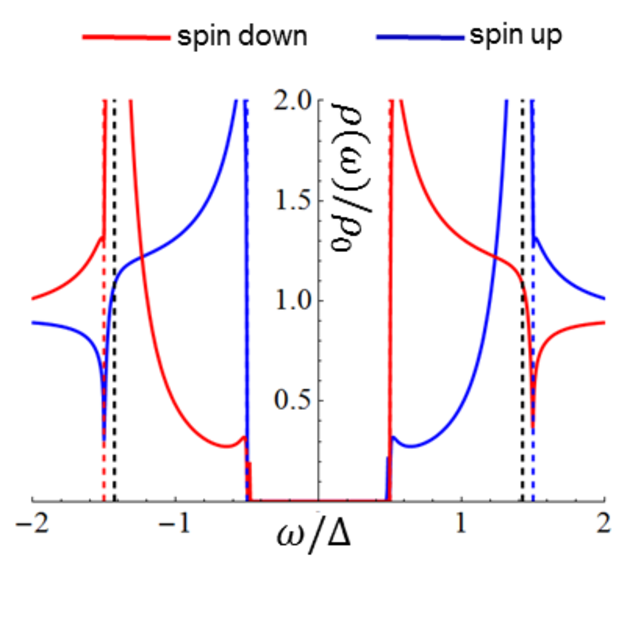
\includegraphics[width=0.25\linewidth]{ApLDOSa} \hspace{0.1cm}
	(b)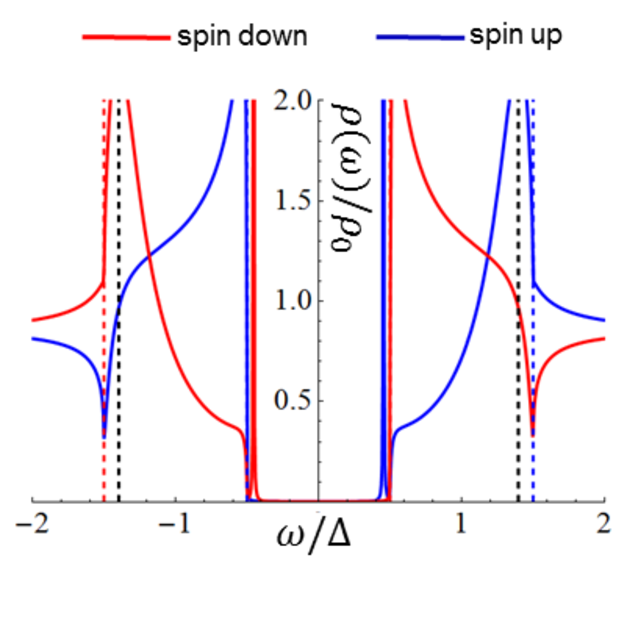
\includegraphics[width=0.25\linewidth]{ApLDOSb} \hspace{0.1cm}
	(c)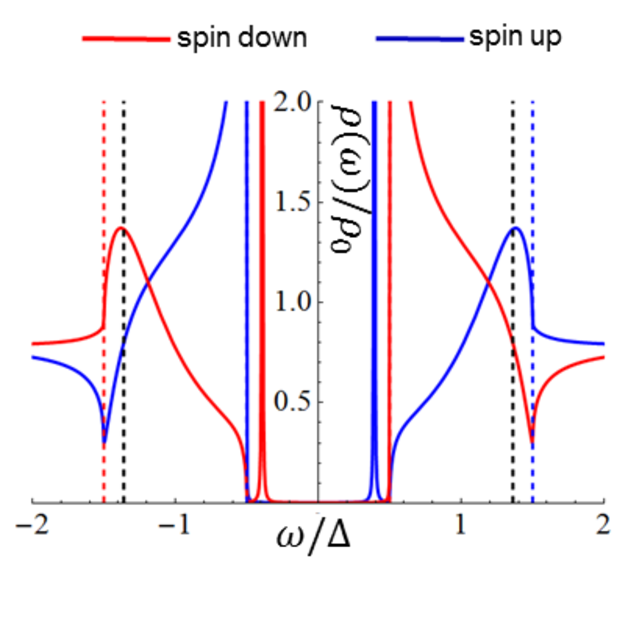
\includegraphics[width=0.25\linewidth]{ApLDOSc} 
	\caption{(Color online) Spin-polarized local density of states (SP-LDOS)  at the core of the skyrmion. The consequent panels correspond to increasing skyrmion size (a) $R = 1.1 p_F^{-1}$, (b) $R = 1.2 p_F^{-1}$, (c) $R = 1.3 p_F^{-1}$. Other parameters are the same as in Fig.~\ref{fig:LDOS}. } \label{fig:ApLDOS}
\end{figure*}
%%%%%%%%%%%%%%%%%%%%%%%%%%%%%%%%%%%%%%%%%%%%%%%%%%%%%%%%%%%%%%%%%%%%%%%%%%


In this section, we give an analytic treatment of the skyrmion-induced bound states using the T-matrix approximation. Starting from the Hamiltonian (\ref{ham}) in the second-quantized form, we write the Bogolyubov-de Gennes (BdG) Hamiltonian as 
\begin{align}
	& H_{\rm BdG} = H(\bm p) + V(\bm r),\quad {\rm where} \nonumber \\
& H(\bm p) = \xi(\bm p)\tau_z+\Delta \tau_x - \bm S(\infty)\cdot\bm\sigma,\quad \bm S(\infty) = -S\,\hat{\bm z}, \nonumber\\
& V(\bm r) = -\left[ \bm S(\bm r)-\bm S(\infty)\right]\cdot\bm\sigma \label{v0}
\end{align}
The momentum-dependent part $H(\bm p)$ describes a superconductor coupled to a spatially uniform ferromagnetic vector $\bm S(\infty)$, whereas the position-dependent piece $V(\bm r)$ describes the local perturbation due to the skyrmion. Physically, the superconducting coherence legth $\xi\sim 100$\,nm is much greater than the radius of the skyrmion $R\sim 10$\,nm (plug the real numbers from Wiesendanger papers), i.e. $\xi\gg R$. Therefore, the superconductivity does not ``resolve'' the fine details of the skyrmionic configuration of the field  $\bm S(\bm r)$, but rather ``sees'' its long-wavelength characteristics such as the moments described by Eqs.~(\ref{S0}) and (\ref{S1}). Motivated by this logic, we substitute the original skyrmionic field $\bm S(\bm r)$ by its local version 
\begin{equation}
	\bm S(\bm r) - \bm S(\infty) = \left[ S_{\rm e}\, \hat{\bm z} - S_{\rm m}\, \bm \nabla\right] \delta^2(\bm r).
	\label{S}
\end{equation}
By plugging Eq.~(\ref{S}) in the equations for the moments~(\ref{S0}) and (\ref{S1}), one can verify the definitions of the effective $S_{\rm e}$ and monopole $S_{\rm m}$ moments.  The latter simplified field $\bm S(\bm r)$ is especially convenient for the T-matrix calculation, which we now proceed to. We take into account (\ref{S}) and calculate the Fourier transform of Eq.~(\ref{v0})  
\begin{equation}
	V(\bm p) = -S_{\rm e}\,\sigma_z +  i \,S_{\rm m} \, \bm \sigma\cdot \bm  p,
	\label{vp}
\end{equation}
using which we write an intergal equation for the T-matrix
\begin{align}
	T\left(\bm p^{1},\bm p^{2}\right) &= V \left(\bm p^{1}-\bm p^{2}\right) \nonumber \\
	& +\int d^2 p'\, V\left(\bm p^{1}-\bm p'\right) g(\omega,\bm p')  T\left(\bm p',\bm p^{2}\right).
	\label{integEq}
\end{align}
Here, the bare Green's function of the superconductor is defined as 
\begin{align}
	g(\omega,\bm p) = \frac{1}{\omega-H(\bm p)} = \frac{1}{\omega-\xi(\bm p)\tau_z-\Delta \tau_x - S\sigma_z}.
\end{align}
Since in the case of the superconductivity we are interested in the scatterings close to the Fermi surface, we use $\bm p^{1} = p_F\, \bm n^{1}$ and $\bm p^{2} = p_F \,\bm n^{2}$, where the in-plane unit vectors $\bm n^{1}$ and $\bm n^{2}$ determine the direction of scattering on the Fermi surface.  Then, we seek the T-matrix in the following form
\begin{align}
	T\left(\bm n^{1},\bm n^{2}\right) &= A + B_i n^{1}_i + C_i n^{2}_j + D_{ij} n^{1}_i n^{2}_j, \label{ansatz}
\end{align}
where  $A,B_i,C_i$ and $D_{ij}$ are the matrices in the four-components space $\sigma\otimes\tau$. We substitute ansatz~(\ref{ansatz}) in the integral Eq.~(\ref{integEq}) and find the T-matrix
\begin{widetext}
\begin{equation}
	T\left(\bm n^{1},\bm n^{2}\right) = \frac{-S_{\rm e}\sigma_z+S^2_{\rm m}p_F^2\bar g_{0}(\omega)+i\,S_{\rm m}\,p_F \,  \bm \sigma\cdot(\bm n^{2}- \bm n^{1}) +S^2_{\rm m}\, p^2_F \, \bar g_{0}(\omega)\,\left(\bm \sigma\cdot\bm n^{2}\right)\,\left(\bm \sigma\cdot \bm n^{1}\right)}{1+S_{\rm e}\sigma_zg_{00}-S^2_{\rm m}p_F^2\,\bar g_{0}(\omega)\, g_{0}(\omega)},
\end{equation}
\end{widetext}
where the Green's function on-site matrix element in the real space is denoted as 
\begin{align}
	g_{0}(\omega) &   =\int d^2 p\, g(\omega,\bm p)  	\label{g0} \\
	 & =-\pi\rho\sum_{\lambda = \pm 1} \frac{1+\lambda\sigma_z}{2}\,\frac{\omega-\lambda S+\Delta\tau_x}{\sqrt{\Delta^2-\left( \omega-\lambda S \right)^2}}, \nonumber \\
	 \bar g_{0}(\omega) & = \frac{1}{2} \sum_{j=x,y}\sigma_j\, g_{0}(\omega)\, \sigma_j.\label{bg0}
\end{align}
For brevity, $\bar g_{0}$ denotes the Green's function obtained from $g_{00}$ by replacing $\sigma_z \rightarrow - \sigma_z$ according to Eq.~(\ref{bg0}). The density of states per spin is denoted as $\rho = m/2\pi$.
%%%%%%%%%%%%%%%%%%%%%%%%%%%%%%%%%%%%%%%%%%%%%%%%%%%%%%%%%%%%%%%%%%%%%%%%%%%%%
\subsection{LDOS} \label{sec:LDOS}
%%%%%%%%%%%%%%%%%%%%%%%%%%%%%%%%%%%%%%%%%%%%%%%%%%%%%%%%%%%%%%%%%%%%%%%%%%%%%
So, in the presence of the skyrmion, the Green's function becomes
\begin{align}
	G(\omega,\bm p^1,\bm p^2) =& g(\omega,\bm p^1)\,(2\pi)^2\delta(\bm p^1-\bm p^2) \nonumber \\ 
	          &  +g(\omega,\bm p^1) T(\bm p^1,\bm p^2) g(\omega,\bm p^2),
	\label{G}
\end{align}
using which the spin-polarized local density of states (LDOS) can be expressed
\begin{align}
	\rho_s(\omega,\bm r) = -&\frac{1}{\pi}\,{\rm Im}\lim_{\omega\rightarrow \omega+i\delta}{\rm\,Tr} \left[ \frac{1+\tau_z}{2}\,\frac{1+\sigma_s}{2} \right. \label{rhor} \\
	&\left.\int \frac{d^2p^1\,d^2p^2}{\left( 2\pi \right)^4} e^{i\left( \bm p^1-\bm p^2 \right)\bm r} G(\omega,\bm p^1,\bm p^2)\right]\, \nonumber 
\end{align}
where $s=x,y,z$ denotes the spin quantization axis. It can be easily evaluated for instance at the skyrmion core, i.e. at $\bm r=0$,
\begin{align}
	& \rho_s(\omega,0) = -\frac{1}{\pi}\,{\rm Im}\lim_{\omega\rightarrow \omega+i\delta}{\rm \,Tr} \left\{  \frac{1+\tau_z}{2}\,\frac{1+\sigma_s}{2}  \right. \label{spldos} \\
	&\left.\left[g_0(\omega)+g_0(\omega)  \frac{-S_{\rm e}\sigma_z+S^2_{\rm m}p_F^2\bar g_{0}(\omega)}{1+S_{\rm e}\sigma_zg_{00}-S^2_{\rm m}p_F^2\,\bar g_{0}(\omega)\, g_{0}(\omega)} g_0(\omega)  \right]\right\}\, \nonumber 
\end{align}

%%%%%%%%%%%%%%%%%%%%%%%%%%%%%%%%%%%%%%%%%%%%%%%%%%%%%%%%%%%%%%%%%%%%%%%%%%%%%
\subsection{Spatial wave function} \label{sec:wf}
%%%%%%%%%%%%%%%%%%%%%%%%%%%%%%%%%%%%%%%%%%%%%%%%%%%%%%%%%%%%%%%%%%%%%%%%%%%%%



%%%%%%%%%%%%%%%%%%%%%%%%%%%%%%%%%%%%%%%%%%%%%%%%%%%%%%%%%%%%%%%%%%%%%%%%%%%%%
%\bibliographystyle{apsrev4-1}
\bibliography{Skyrmion}
%%%%%%%%%%%%%%%%%%%%%%%%%%%%%%%%%%%%%%%%%%%%%%%%%%%%%%%%%%%%%%%%%%%%%%%%%%%%%



\end{document}
